\documentclass[a4paper,10pt]{article}
\usepackage[paper=a4paper, hmargin=1.5cm, bottom=1.5cm, top=3.5cm]{geometry}

\usepackage[utf8]{inputenc} %Codificacion de caracteres, para poder usar acentos, etc.
\usepackage[T1]{fontenc}
\usepackage[spanish]{babel}
\usepackage{xspace}
\usepackage{xargs} %Para crear funciones con muchos argumentos
\usepackage{ifthen}
\usepackage{aed2-tad,aed2-symb,aed2-itef,caratula} %Macros de Algo2
\usepackage{algorithm}% http://ctan.org/pkg/algorithms
\usepackage{algpseudocode} % Para algorritmia
%\usepackage{algorithmic} %paquete para hacer pseudocodigo

\usepackage{titlesec}%http://foro-c.com/blog/latex-formato-de-titulos-de-capitulos-secciones-etc/
\usepackage{graphicx} %Inlcuir imagenes.
\usepackage{setspace}
\usepackage{fancyhdr}
\usepackage[colorlinks=true, linkcolor=blue]{hyperref} %Links para el indice.
\usepackage{float} %Insercion de imagenes flotantes
\usepackage{ stmaryrd }

\usepackage{caption}
\usepackage{subcaption}

\newcommand{\moduloNombre}[1]{\textbf{#1}}

\let\NombreFuncion=\textsc
\let\TipoVariable=\texttt
\let\ModificadorArgumento=\textbf
\newcommand{\res}{$res$\xspace}
\newcommand{\tab}{\hspace*{7mm}}

\newcommandx{\TipoFuncion}[3]{%
  \NombreFuncion{#1}(#2) \ifx#3\empty\else $\to$ \res\,: \TipoVariable{#3}\fi% nombreFuncion(parametros) -> res:(Tipo)
}
\newcommand{\In}[2]{\ModificadorArgumento{in} \ensuremath{#1}\,: \TipoVariable{#2}\xspace}
\newcommand{\Out}[2]{\ModificadorArgumento{out} \ensuremath{#1}\,: \TipoVariable{#2}\xspace}
\newcommand{\Inout}[2]{\ModificadorArgumento{in/out} \ensuremath{#1}\,: \TipoVariable{#2}\xspace}
\newcommand{\Aplicar}[2]{\NombreFuncion{#1}(#2)}

\newlength{\IntFuncionLengthA}
\newlength{\IntFuncionLengthB}
\newlength{\IntFuncionLengthC}
%InterfazFuncion(nombre, argumentos, valor retorno, precondicion, postcondicion, complejidad, descripcion, aliasing)
\newcommandx{\InterfazFuncion}[9][4=true,6,7,8,9]{%
  \hangindent=\parindent
  \TipoFuncion{#1}{#2}{#3}\\%
  \textbf{Pre} $\equiv$ \{#4\}\\%
  \textbf{Post} $\equiv$ \{#5\}%
  \ifx#6\empty\else\\\textbf{Complejidad:} #6\fi%
  \ifx#7\empty\else\\\textbf{Descripcion:} #7\fi%
  \ifx#8\empty\else\\\textbf{Aliasing:} #8\fi%
  \ifx#9\empty\else\\\textbf{Requiere:} #9\fi%
}

\newenvironment{Algoritmos}{%
  \vspace*{2ex}%
  \noindent\textbf{}%
  \vspace*{2ex}%
}{}


\newcommand{\Titulo}[1]{
  \vspace*{1ex}\par\noindent\textbf{\large #1}\par
}

\newcommand{\DRef}{\ensuremath{\rightarrow}}

\newcommandx{\Algoritmo}[4]{%
	\noindent\TipoFuncion{#1}{#2}{#3}
	\begin{algorithmic}[1]
	#4
	\end{algorithmic}
}%

\newcommand{\nom}[1]{\NombreFuncion{#1}}

\newcommand{\comp}[1]{\hfill \ensuremath{O(#1)}}
\newcommand{\compTot}[1]{\hfill \textbf{Complejidad Total: }\ensuremath{O(#1)}}

\sloppy

\hypersetup{%
 % Para que el PDF se abra a pagina completa.
 pdfstartview= {FitH \hypercalcbp{\paperheight-\topmargin-1in-\headheight}},
 pdfauthor={C\'atedra de Algoritmos y Estructuras de Datos III - DC - UBA},
 pdfkeywords={},
 pdfsubject={}
}

\parskip=5pt % 10pt es el tamano de fuente

% Pongo en 0 la distancia extra entre itemes.
\let\olditemize\itemize
\def\itemize{\olditemize\itemsep=0pt}

% Acomodo fancyhdr.
\pagestyle{fancy}
\thispagestyle{fancy}
\addtolength{\headheight}{1pt}
\lhead{Algoritmos y Estructuras de Datos III}
\rhead{TP 3}
% \lhead{Algoritmos y Estructuras de Datos II}
% \rhead{$1^{\mathrm{do}}$ cuatrimestre de 2006}
%\cfoot{\thepage /\pageref{LastPage}}
%\renewcommand{\footrulewidth}{0.4pt}

\author{}
\date{01-07-2013}
\title{Trabajo}

\begin{document}
 
\materia{Algoritmos y Estructuras de Datos III}
\subtitulo{}
\titulo{Trabajo Pr\'actico 3}
\grupo{}

\integrante{Laura Muiño}{399/11}{mmuino@dc.uba.ar}
\integrante{Mart\'in Santos}{413/11}{martin.n.santos@gmail.com}
\integrante{Luis Toffoletti}{827/11}{luis.toffoletti@gmail.com	}
\integrante{Florencia Zanollo}{934/11}{florenciazanollo@hotmail.com}

\maketitle
\tableofcontents

\newpage

%\section{Algoritmo_Exacto}

%\newpage

\section{Algoritmo Goloso}
\subsection{Explicación del algoritmo implementado}
La heurística golosa que implementamos consiste en buscar el nodo de mayor grado del grafo. A partir de ese nodo v, se construye una clique de frontera máxima de la siguiente manera:

\begin{algorithm}[H]
\caption{Goloso}\label{ej2}
\begin{algorithmic}[1]
\Procedure{Goloso}{$G=(V,E)$}
	\State clique  $\shortleftarrow$ $\{$v nodo de mayor grado$\}$
	\While{ $\{Aumente frontera\}$ }
		\State $\{$Buscar nodo u$\}$ tal que u $\in$ nodos de la frontera y $ d(u) \ge d(p)$ $ \forall p \neq u $ y forme clique con nodos de clique
		\State clique $\cup$ $\{u\}$
	\EndWhile
	\State return |frontera|, |clique|, clique 
\EndProcedure
\end{algorithmic}
\end{algorithm}
Veamos con más detalle ciertos procedimientos para facilitar luego el análisis de complejidad.

Linea 4: Conseguir nodo candidato es básicamente intersecar los adyacentes de cada nodo de la clique que se tiene hasta el momento y luego tomar aquel de mayor grado. ¿Por qué la intersección de los adyacentes?. Porque me aseguro de obtener los nodos de la frontera que sean adyacentes a los nodos de la clique, lo que me permite agrandarla.
¿Por qué el de mayor grado?. Porque será el que mas nodos aporte a la nueva clique del resto de los nodos obtenidos en la intersección.
La intersección entre dos grupos de elementos consiste en recorrer uno de estos grupos y devolver aquellos que tienen coincidencias contra todos los elementos del otro grupo.

Linea 7: Calcular el tamaño de la \textit{frontera} consiste en sumar la cantidad de adyacentes de cada nodo de la clique y restar a este último número resultate las aristas de la clique (que son$ \displaystyle\frac{n(n-1)}{2}$).  

%%%%%%%%%%%%%%%%%%%%%%%%%%%%%%%%%%%%%%%%%%%%%%%%%%%%%%%%%%%%%%%%%%%%%%%%%%%%%%%%%%%%%%%%%%%%%%%%%%%%%%%%%%%%%%%%%%%%%%%%%%%%%%%%%%%%%%%%%%%%%%
%%%%%%%%%%%%%%%%%%%%%%%%%%%%%%%%%%%%%%%%%%%%%%%%%%%%%%%%%%%%%%%%%%%%%%%%%%%%%%%%%%%%%%%%%%%%%%%%%%%%%%%%%%%%%%%%%%%%%%%%%%%%%%%%%%%%%%%%%%%%%%

\subsection{Complejidad}
Veremos la complejidad de la heurística golosa siguiendo paso a paso el algoritmo:
\begin{itemize}
 \item En la linea 2, conseguir el nodo de mayor grado es O(n) pues se recorren todos los nodos.
 \item En la linea 3, se hacen a lo sumo n iteraciones (puede que la clique de frontera máxima sea el grafo entero), luego O(n).
 \item En la linea 4, buscar el nodo candidato tiene una complejidad O($n^{3}$).
\end{itemize}

Luego podemos concluir que la complejidad de la heurística es polinómica (más precisamente O($n^{4}$)). 

\begin{center}
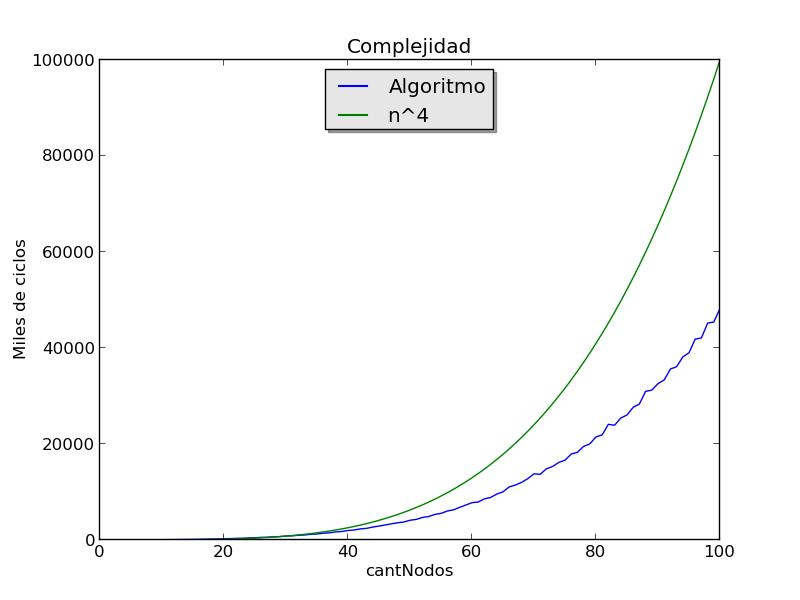
\includegraphics[scale=0.5]{goloso/grafico.jpg} 
\end{center}
El gráfico de complejidad fue realizado en base a grafos completos para asegurarnos que el algorítmo no supere la cota de complejidad en casos con muchas aistas y muchos nodos.
%%%%%%%%%%%%%%%%%%%%%%%%%%%%%%%%%%%%%%%%%%%%%%%%%%%%%%%%%%%%%%%%%%%%%%%%%%%%%%%%%%%%%%%%%%%%%%%%%%%%%%%%%%%%%%%%%%%%%%%%%%%%%%%%%%%%%%%%%%%%%%
%%%%%%%%%%%%%%%%%%%%%%%%%%%%%%%%%%%%%%%%%%%%%%%%%%%%%%%%%%%%%%%%%%%%%%%%%%%%%%%%%%%%%%%%%%%%%%%%%%%%%%%%%%%%%%%%%%%%%%%%%%%%%%%%%%%%%%%%%%%%%%

\subsection{Casos nefastos}

Los casos en que esta heurística falla, son aquellos en que el nodo de mayor grado del grafo no se encuentra dentro de la clique que se busca. 
¿Cuán mala puede ser? Tan mala como uno quiera, basta formar, por ejemplo, una estrella con el nodo central de grado máximo y una clique de fontera máxima con tamaño menor al grado máximo. Como ejemplo ilustrativo, mirar la siguiente imagen.
\begin{center}
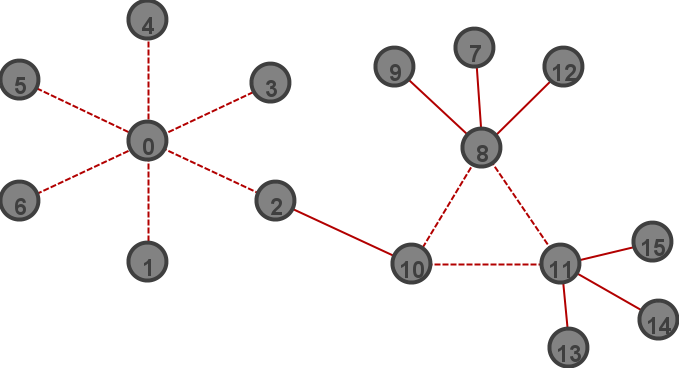
\includegraphics[scale=0.5]{goloso/labl.png} 
\end{center}


%\section{Algoritmo_Busqueda_Local}
%\input{}
%\newpage

\end{document}
